\documentclass{article}
\usepackage[utf8]{inputenc}

\title{Problem Set 6}
\author{Karley Nadolski}
\date{March 2021}

\usepackage{graphicx}
\usepackage{hyperref}

\begin{document}

\maketitle

\section{Introduction}
For these visualizations, I used a data set from \href{https://www.kaggle.com/jsphyg/weather-dataset-rattle-package}{Kaggle} with 10 years of daily weather observations from 49 different weather centers across Australia. Variables include MaxTemp, MinTemp, Rainfall, as well as more specific information about cloud covering or wind gusts. 

Because it was presented for data science use, this dataset was already pretty clean when I downloaded it as a CSV file. For general cleaning, I mainly went through and trimmed down the dataframe to exclude any of the columns that were completely filled with NA values. Other than that, the most of the cleaning/data manipulation that I did was specific to the visualization that I wanted to create. That being said, the dataset contains 145,560 observations on 23 different variables. Most of my cleaning across the three graphics that I made included debating how to to subset the information so as not to be visually overwhelming. I will more specifically outline each process when introducing the three separate figures below. 

\section{Figure 1 Explanation} 
In Figure 1, I wanted to show the relationship between temperature and rainfall amounts. This was the only graphic where I didn't significantly subset the thousands of observations. Instead, I wanted to create a sort of "distribution" that could broadly show the relationship of interest over the entire study region. I made each point take on a color that represented its location. Because of the sheer number of data points the color is not super meaningful, but it could be helpful in recognizing any spatial trends in the data (specifically with the teal points close to the origin). In the future, I would probably skip this addition of color/location or change it so there wasn't 49 different color options by charting location regionally instead of locally. Still, I thought this graphic was interesting and could be useful in the right context. 

\begin{figure} {h!}
\centering
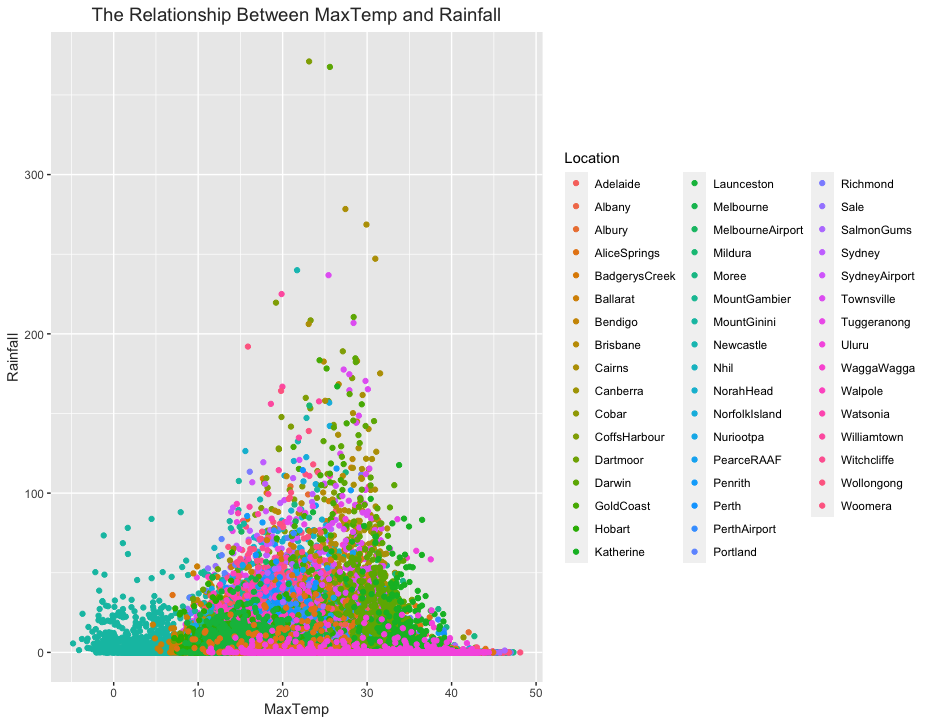
\includegraphics[scale=0.3]{PS6a_Nadolski.png}
\caption{Relationship between high temperature and rainfall}
\label{fig:a}
\end{figure}

\section{Figure 2 Explanation}
In Figure 2, I wanted to show average rainfall by location to directly compare locations included in the dataset. To do this, I created a for loop that calculated the average rainfall by location and organized it in a new dataset. This visualization is based off of the information in that dataset. Because there are 49 unique locations included in this dataset, I decided to subset the data further to only include the locations with the 10 highest average rainfall amounts. I made the decision to make the chart easier to take in visually, as the version with 49 locations was difficult to read and interpret. In the future, I want to figure out how to format the Y-axis to have regular intervals that aren't determined by the data. Visually, the chart communicates the difference in rainfall across the 10 locations, but I worry that the scale isn't exactly correct. 

\begin{figure} [h!]
\centering
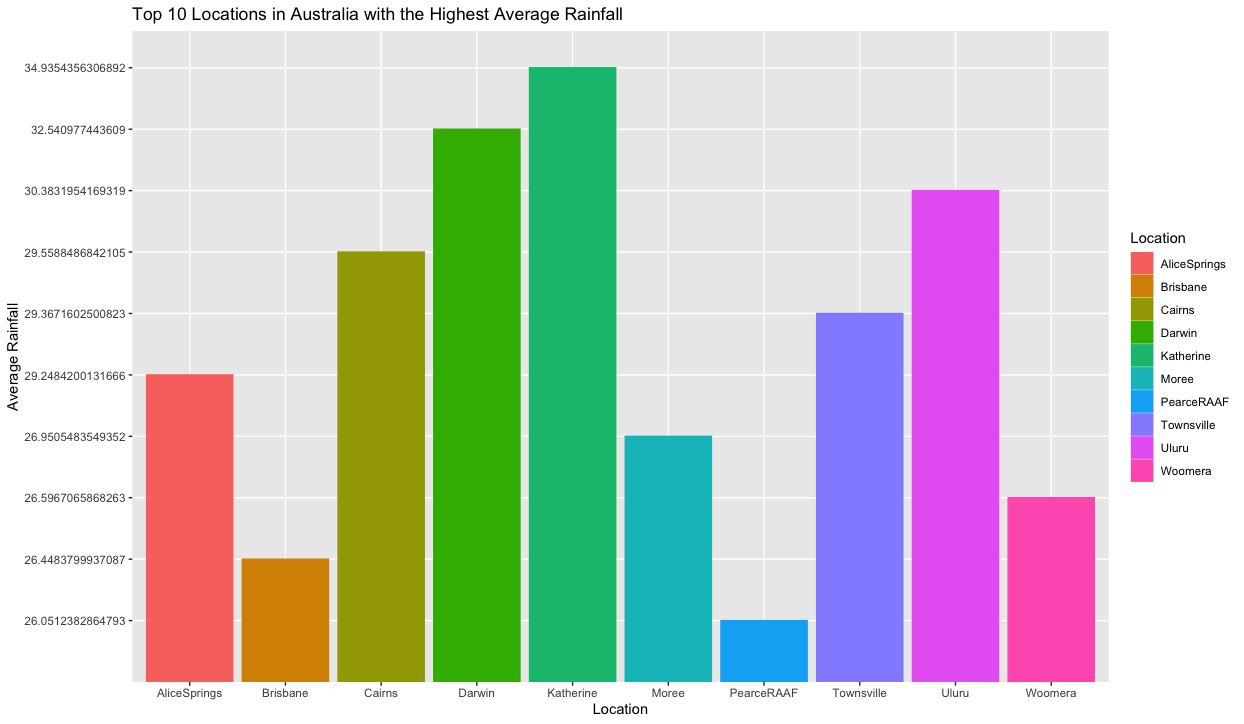
\includegraphics[scale=0.275]{PS6b_Nadolski.png}
\caption{Top 10 rainiest locations in Australia}
\label{fig:b}
\end{figure}




\section{Figure 3 Explanation}
In Figure 3, I wanted to choose one location and visually show the daily high temperature over the study period. I chose to focus on Katherine, Australia. This was the location that I found to have the highest average rainfall. To code this graphic, I created a new, smaller, dataset that only included information where Location == "Katherine". This graphic shows seasonality (obviously), but it also shows how the highs of one year related to the highs of the next (and similarly with the lows). In my opinion, this graphic would probably be the most useful as it is now for those studying weather, climate, or Katherine, Australia. 

\begin{figure} [!h]
    \centering
    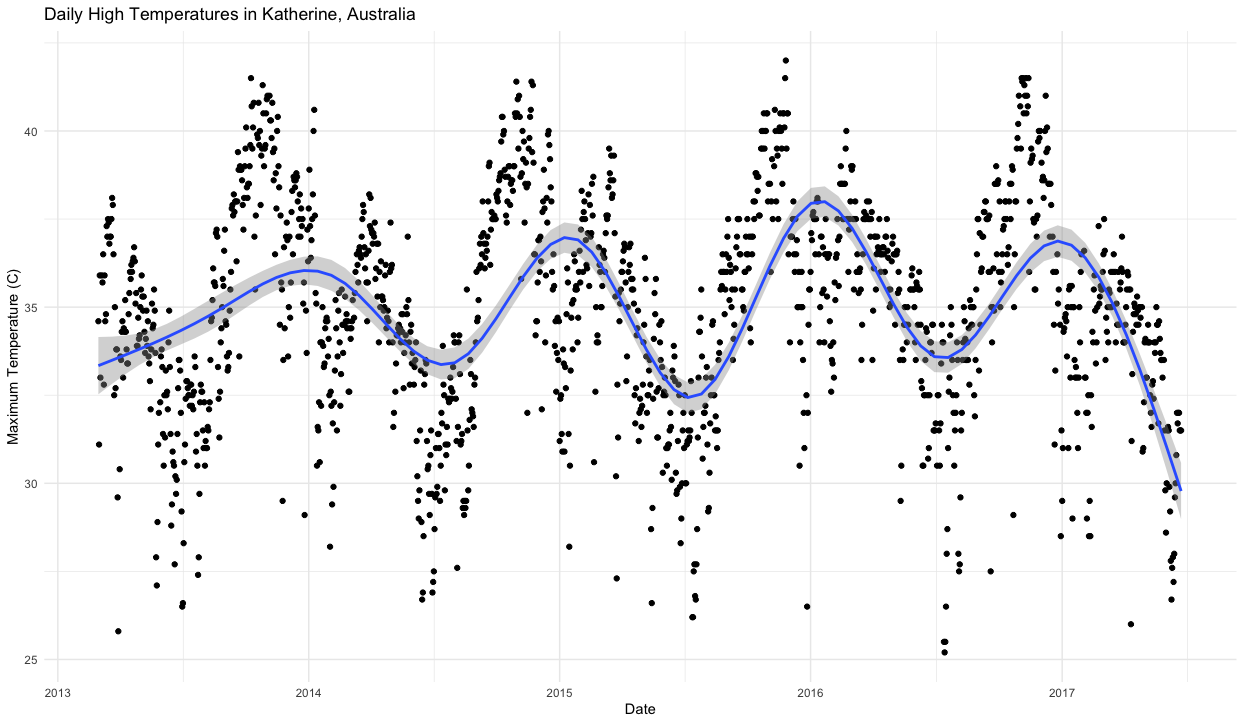
\includegraphics[scale=0.275]{PS6c_Nadolski.png}
    \caption{Daily high temperatures in Katherine, Australia}
    \label{fig:c}
\end{figure}


\bibliographystyle{plain}
\bibliography{references}
“Rain in Australia.” Accessed March 18, 2021. \url{https://kaggle.com/jsphyg/weather-dataset-rattle-package}

\end{document}
